\documentclass[11pt]{article}
\usepackage[letterpaper,margin=1in]{geometry}
\usepackage{color}
\usepackage[dvipdfmx]{graphicx}
\usepackage{amsbsy}
\usepackage{amsmath}
\usepackage{adjustbox}
\usepackage{url}
%\usepackage{floatrow}
\usepackage[font=small,labelfont=bf,tableposition=top]{caption}
\DeclareCaptionLabelFormat{tableonly}{\tablename~\thetable}
%\newfloatcommand{capbtabbox}{table}[][\FBwidth]


\newcommand{\argmax}{\mathop{\rm arg~max}\limits}

\begin{document}
\vspace{-1cm}
\title{\vspace{-2ex}Project proposal for the ML class final project\vspace{-2ex}}
\author{Yoshinari Fujinuma\vspace{-2ex}}
\date{\vspace{-2ex}}
\maketitle

\vspace{-0.5cm}

\section{Debugging Tweet2vec (to build a better character representation?)}

Two problems of Tweet2vec \cite{dhingra-EtAl:2016:P16-2} (i.e. bidirectional GRU for hashtag prediction):

\begin{enumerate}
 \setlength\itemsep{0.01em}
 \item  Since Twitter users are lazy, many of the relevant hashtags are not added by users. Therefore, hashtag prediction on a hold out set is not a good evaluation.
 \item Tweet2vec is black box and we are not sure whether the model is learning a correct model in any given training data. (Similar to Chirstmas vs. fever problem for flu classifier \cite{Paul-2016} .)
\end{enumerate}

{\bf Objective of the project}: Solve the problem 2.

Comparing Figure 1 and Figure 2, whether the model is correctly predicting from human-intuitive feature is not apparaent in Figure 2. %effect is not made transparenet.
To solve the problem, we would like to start off from trying recently proposed interpretable methods:
\begin{enumerate}
 \item Model-agnostic interpretation (e.g., LIME \cite{Ribeiro:2016})
 \item Attention mechanism \cite{luong-pham-manning:2015:EMNLP}
\end{enumerate}

%\begin{figure}[htb]
%  %\vspace{-1.1cm}
%  \begin{center}
%   \begin{tabular}{c}
%    \begin{minipage}{0.5\hsize}
%     \begin{center}
%     \scalebox{0.25}
%     %\scalebox{0.33}
%      %{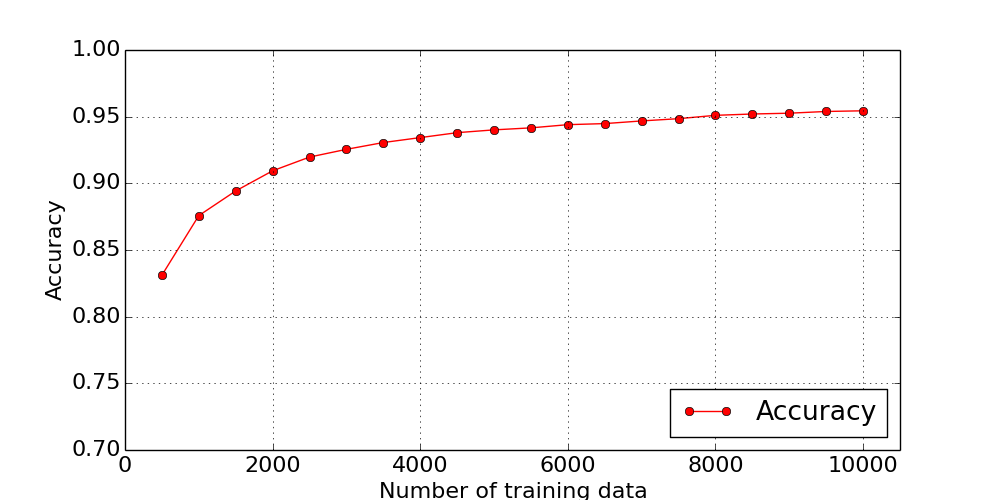
\includegraphics[]{figure_1.png}}
%      {\includegraphics[]{pictures/RNM_attention_figure.png}}
%   
%      \caption{The attention figure from the RMN paper. }
%      \label{fig:learning_rate}
%     \end{center}
%    \end{minipage}
%
%    \begin{minipage}{0.01\hsize}
%    \end{minipage}
%
%    \begin{minipage}{0.5\hsize}
%     \begin{center}
%      %\scalebox{0.33}
%      \scalebox{0.25}
%      {\includegraphics[]{pictures/tweet2vec_figure.png}}
%      \caption{\label{stopping_criterion}Stopping criterion.}
%     \end{center}
%    \end{minipage}
%
%  \end{tabular}
% \end{center}
%\vspace{-0.5cm}
%\end{figure}

\begin{figure}[htb]
  \begin{center}
     \scalebox{0.3}
      %{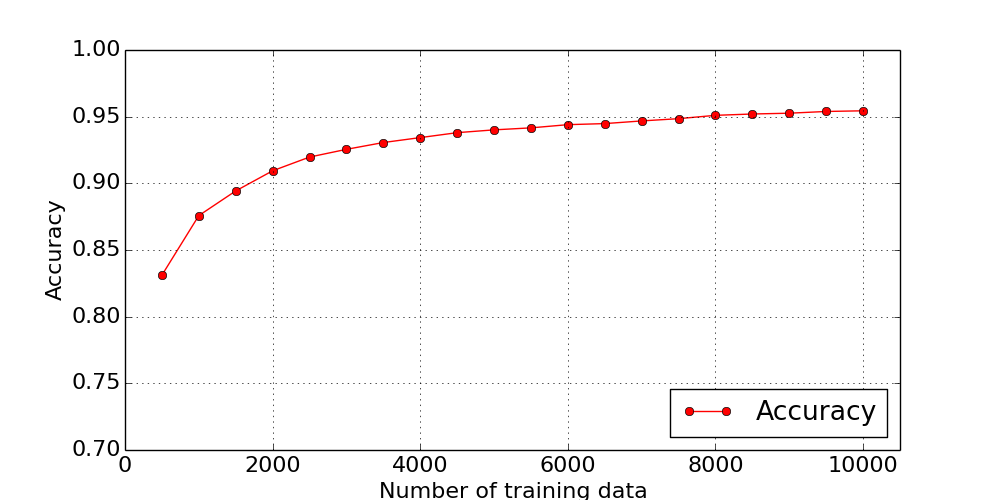
\includegraphics[]{figure_1.png}}
      {\includegraphics[]{pictures/tweet2vec_figure.png}}
      \caption{The attention figure from the Recurrent Memomry Network paper. }
      \label{fig:learning_rate}
     \end{center}
\vspace{-0.5cm}
\end{figure}



\begin{figure}[htb]
  \begin{center}
     \scalebox{0.3}
      %{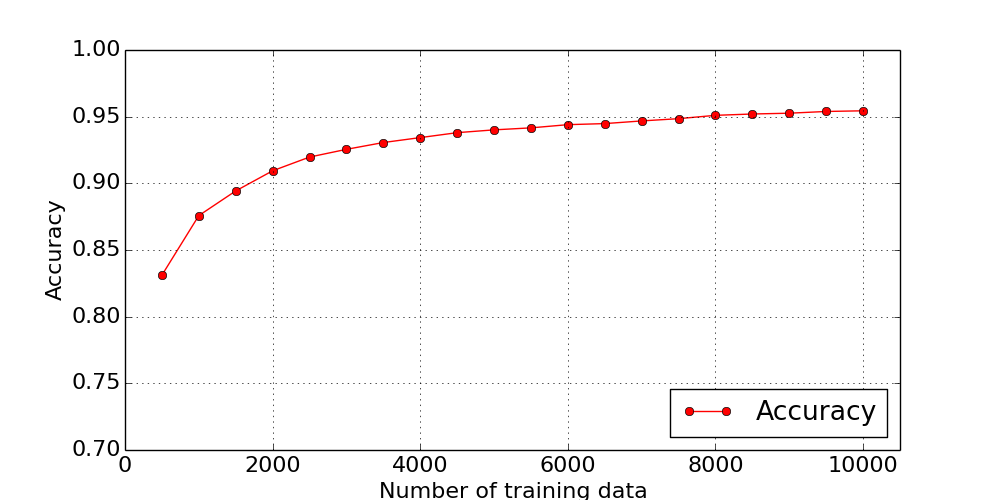
\includegraphics[]{figure_1.png}}
      {\includegraphics[]{pictures/RNM_attention_figure.png}}
   
      \caption{The prediction example from tweet2vec paper \cite{dhingra-EtAl:2016:P16-2}. }
      \label{fig:learning_rate}
     \end{center}
\vspace{-0.5cm}
\end{figure}

%\section{Curriculum Learning and Tweet2vec}

\bibliographystyle{plain}
\bibliography{project_proposal}

\end{document}
